\documentclass[conference]{IEEEtran}

\usepackage{makeidx}  % allows for indexgeneration
\usepackage{graphicx}
\usepackage{indentfirst}
\usepackage{hyperref}
\usepackage{verbatim}
\usepackage{balance}
\usepackage{amsmath}

\begin{document}
\sloppy
\IEEEoverridecommandlockouts
%
% paper title
% can use linebreaks \\ within to get better formatting as desired
\title{From Abstract Parsing to Abstract Translation {\thanks{This work is licensed under the Creative Commons Attribution License.}}}

% author names and affiliations
% use a multiple column layout for up to three different
% affiliations
\author{\IEEEauthorblockN{Semen Grigorev}
\IEEEauthorblockA{St. Petersburg State University\\
198504, Universitetsky prospekt 28\\
Peterhof, St. Petersburg, Russia\\
Email: rsdpisuy@gmail.com}
\and
\IEEEauthorblockN{Iakov Kirilenko}
\IEEEauthorblockA{St. Petersburg State University\\
198504, Universitetsky prospekt 28\\
Peterhof, St. Petersburg, Russia\\
Email: jake@math.spbu.ru}}

\maketitle

\begin{abstract}
String-embedded language transformation is one of the problems which can be faced during 
database and information system migration. The conventional solution which
is provided by a number of tools is based on run-time translation. We present a static 
\emph{abstract translation} approach which originates from the \emph{abstract parsing} 
technique~\cite{AbstrParsing} initially developed for syntax analysis of string-embedded 
languages. We present abstract translation algorithm and some optimization techniques, and
discuss the results of its evaluation on a real-world industrial application.

\end{abstract}

\IEEEpeerreviewmaketitle



\section{Introduction}

Complex information systems are often implemented using more than one programming language. 
Sometimes this variety takes form of one \emph{host} and one or few \emph{string-embedded}
languages. Textual representation of clauses in a string-embedded language is built at 
run time by a host program and then analyzed, compiled or interpreted by a dedicated 
runtime component (database, web browser etc.) Most general-purpose programming languages 
may play role of the host; one of the most evident examples of string-embedded language is 
dynamic SQL which was specified in ISO SQL standard in 1992~\cite{ISO} and since then is 
supported by the majority of DBMS. 

%allow to use string-embedded languages: dynamically build 
%expressions in other languages as string values and evaluate them with intended processor 
%(database, web browser, or interpreter). 
%In the current work we use dynamic SQL as an 
%example of string-embedded languages. The mechanism of dynamic SQL queries contraction 
%and execution was specified in ISO SQL standard in 1992~\cite{ISO} and most DBMS
%support this. 

%Dynamically constructed expressions is a string expressions in any programming language 
%and for compiler they are just string constants. 

String-embedded languages may help to compensate the lack of expressivity of general-purpose
language in a domain-specific settings or to integrate heterogeneous components of large system;
however this approach comes with some price. In particular even the syntax analysis of 
string-embedded part of a system is undecidable in general case since its source code
is represented implicitly using string-manipulation primitives, procedures and libraries, and
generated ``on the fly''. In a na\"ive implementation syntax analysis of embedded clauses is
completely outsourced to the runtime environment which postpones many errors from being 
discovered prior to execution and thus compromises the ideas of code safety and static control.

\emph{Abstract parsing} is the approach which was developed to overcome the 
aforementioned deficiency. In abstract parsing the source code of a host application is statically 
analyzed to provide some constructive representation of the set of string-embedded language clauses which
can possible be generated at run time~\cite{AbstrParsing,StringExpr}. This representation is then analyzed 
by a certain parsing algorithm which is usually derived from some existing one for plain strings~\cite{Grune}.
Abstract parsing technique is utilized in a number of tools~\cite{JSA,PHPSA,ALVOR1,ALVOR2} for
program analysis and understanding.

While abstract parsing can help in application analysis it cannot handle the case of application
\emph{transformation}. As a practical use case for string-embedded language transformation we can mention
reengineering. During reengineering it is sometimes necessary to migrate from one database management 
system to another; this migration may require a transformation of string-embedded 
clauses. 

One of the options is dynamic translation at run time~\cite{OpenSystemsDBMS}. However this solution
not always desirable. First, it may degrade the performance of the system due to introduction of extra 
processing stage. Next, with dynamic translation the ultimate goals of the reengineering are not achieved 
since some part of the original system escaped transformation. 

Another approach includes translation of stored SQL which is supported by a number of existing production tools 
for database application development~\cite{PLSQL,SwissSQL,SQLWays}. However, these tools do not support 
dynamic SQL translation and thus provide only partial solution. 

%---------

%To solve a problem of dynamic queries translation we should calculate new values for all variables used 
%for queries construction. If we want to create static translator then result of translation should not 
%require any changes after translation is finished. Basic idea is that we should try to apply classical 
%translation techniques to each possible value of dynamic query. So we should build parsing forest and 
%translate each of trees, and calculate new string values based on translation result.

%Semantic equivalent constructions of source and target languages should have similar syntax in order to 
%abstract translation could be applied. If this constraint is not satisfied then solution could not be
%reduced to new values calculation for existing variables. New variable creation may be required and 
%this fact can significantly increase complexity of solution and corresponded analysis.
%---------

%After that we define that input graph tokenization or lexical analysis is the process which convert input graph with string labels on edges (Fig.~\ref{pic1}) 
%to graph with tokens. The same way we define parsing or syntax analysis as the process which produce parsing forest by 
%input graph with edges labeled with tokens. As a result of parsing we have forest where each tree corresponds with query 
%value produced by any path in the input graph. When we describe abstract parsing and translation we assume that input 
%graph tokenization performed successfully.


The contribution of this paper is an approach for \emph{abstract translation}. 
%We present a generalizationof abstract parsing algorithm from~\cite{AbstrParsing} to a translation case. 
Similar to abstract parsing first we perform static analysis to build an approximation for the set of all 
generated clauses. Then our algorithm performs analysis which, unlike abstract parsing, produces 
\emph{parsing forest} --- a family of syntax trees, each of which represents the result of
translation of certain input sequence. New correct assignments for all relevant string values in the host program 
are calculated then. Our approach works only when the source and the target languages are syntactically close 
enough (e.g. when they are two dialects of the same language).  We discuss some heuristic which helps to reduce 
the complexity of the algorithm in many practical cases and present the results of its application for the 
migration of a real-world industrial project from MS-SQL Server 2005 to Oracle 11gR2 platform.

%As a result of abstract translation we should calculate new values for all string variables 
%to ensure   correctness of dynamically constructed expressions in the target system. As we 
%have already mentioned, the problem of static string-embedded language translation is not 
%solved yet.

%and application of the abstract parsing 
%algorithm ~\cite{AbstrParsing} to solve the problem of string-embedded language translation. 
%We describe necessary modifications of basic abstract parsing algorithm to make it applicable 
%to string-embedded language translation in the context of real-world information systems 
%migration. 

%There is a set of tools for string-embedded 
%languages processing, such as PHP String Analyzer ~\cite{PHPSA} or Alvor, but these tools 
%also cannot be used for dynamically constructed expression translation.


%Dynamic queries translation is necessary for information systems reengineering and 
%database applications migration from one database management system to another~\cite{NetDbTransform}. 
%Translation of one dialect of SQL to another is often required during this process. If 
%source code contains dynamic queries then we should guarantee that all string values 
%which are used for dynamic queries building remain correct after translation. By 
%correctness of resulting values we mean that queries formed from them are correct 
%in the context of target DBMS.


%If we want to change execution method or 
%runtime of this expression (e.g. change target database from MySQL to Oracle) then we 
%possibly should transform it. For classical case we have a translator from one language 
%to another, and the process called "translation". Now we want to describe similar process 
%for string-embedded languages and we call it "abstract translation".

 
%Various objects modifications may be performed during information system reengineering 
%for example renaming or dead code elimination . In this case we should guarantee not 
%only syntax correctness of translation results but also semantic correctness in the 
%context of performed environment modifications. 

%For practical usage it is very important that information systems can contain a big 
%number of dynamic queries and each one of them can contains hundreds of 
%branches~\cite{TiunovaUIInt}. The necessity of analyzing all possible values for 
%each query can cause  performance problems and exponential growth of required 
%resources.

%The second possible approach is static translation. It means that it can be done statically 
%as part of information system migration process by the similar way as classical translation. 
%So,  we should generalize translation techniques for application to string embedded languages.  
%As a result of abstract translation we should calculate new values for all string variables 
%to ensure   correctness of dynamically constructed expressions in the target system. As we 
%have already mentioned, the problem of static string-embedded language translation is not 
%solved yet.

%The paper is organized as follows: The next Section introduces and describe abstract parsing. 
%Section~\ref{sec:AbstractTranslation} introduces abstract translation and describes basic 
%ideas of string-embedded language translation algorithm. Section~\ref{sec:Optimizations}
%describes optimizations of abstract translation algorithm discussed in the previous Section. 
%Section~\ref{sec:Evaluation} presents results of proposed algorithm application to real-world 
%migration of the information system which contains more than 2 million lines of code and 
%more than 3000 dynamic SQL queries from MS-SQL Server to Oracle and Section~\ref{sec:Conclusion}
%discuss some problems of abstract translation and possible ways to solve them.


\section{Graph-based Input Representation}
%\label{sec:RelatedWork}

As we mentioned above, the first stage of abstract parsing is static approximation
of relevant string values. Two main representations for approximated values were
used so far. In~\cite{StringExpr,ALVOR1,ALVOR2} the sets of potential string values 
are described using regular expressions; in~\cite{AbstrParsing} approximations are
represented in more implicit form as a solutions of a system of (recursive) dataflow 
equations. 

We did not find a way to scale either of these representations to abstract translation case. 
Instead, we represent the input stream for abstract translation via flow graph with one source and
one sink nodes and string-labeled edges. The labels of edges in this graph represent the results 
of constant propagation so that every path in input graph corresponds to one potential value of dynamic query. 
%Let we define that this path produce corresponded value and we will say that query contains lexical or syntax error if at least 
%one path which produce value with error exists in the corresponding graph. 
Moreover, we perform lexical analysis on graphs which converts the initial string-labeled graphs into
graphs, labeled by tokens.

% After that we define that input graph tokenization or lexical analysis is the process which convert input graph with string labels on edges (Fig.~\ref{pic1}) 
%to graph with tokens. The same way we define parsing or syntax analysis as the process which produce parsing forest by 
%input graph with edges labeled with tokens. As a result of parsing we have forest where each tree corresponds with query 
%value produced by any path in the input graph. When we describe abstract parsing and translation we assume that input 
%graph tokenization performed successfully.

Since any cycle in the input graph generates infinite sequence of tokens which upon translation is turned 
into infinite forest we simplify the graph even more. We replace each cycle with the single repetition. For example in the order to get regular approximation of query value set from code presented below we should build the next regular expression:
$$\text{"select * from "} \cdot (\text{\{tables.get(i)\}}|\varepsilon)^* \cdot \text{";"}$$
and the corresponding finite automaton (see Fig.~\ref{cyclesOrig}). Note that we do not care about approximation for \textit{tables.get(i)} expression because it depends on a constant propagation algorithm. But we will get the graph where cycle replaced with only one repetition of its body. The result of such approximation is presented in Fig.~\ref{cyclesApproximation}.

\begin{verbatim} 
query = "select * from ";
for(int i = 0; i < tables.size(); i++)
{
    if(i != 0) query += ", ";
    query += tables.get(i);
}
query += ";";
\end{verbatim}

\begin{figure}[t]
    \begin{center}
        \includegraphics[width=8cm,height=1.8cm]{../../graphs/cyclesOrig.eps}
        \caption{Correct finite automaton (graph representation)}
        \label{cyclesOrig}        
    \end{center}
\end{figure}



\begin{figure}[t]
    \begin{center}
        \includegraphics[width=8cm,height=0.8cm]{../../graphs/cyclesApproximation.eps}
        \caption{Result of cycles approximation}
        \label{cyclesApproximation}        
    \end{center}
\end{figure}


As you can see, in our example we do not produce strings like \verb|select * from tbl1, tbl2;| or \verb|select * from ;|. So, we can not check it. We process only two strings and all of them are in original infinite set: \verb|select * from tbl1;| and \verb|select * from, tbl1;|. As a result, we do not process all possible values but we process all variables used for query construction and it is enough for such tasks as code highlighting or transformations because all parts of expression are processed. 

Thus the graph becomes cycle-free and we can process all vertices in the topological order. While this drastic simplification is completely heuristic our experience of dynamic SQL translation for real information systems showed that DAG is still a good approximation for practical use.


%In the general case input graph can be arbitrary graph with cycles~\cite{AbstrParsing}. Cycles in the input graph may 
%be cause of infinite parsing. ut we have not found any practice implementations with problem of cycles processing fully 
%solved. We have found only two known implementations of abstract parsing: Alvor\footnote{Alvor is an Eclipse IDE plug-in 
%for statically checking of string-embedded SQL queries in Java programming language. This plug-in is based on LALR and GLR 
%abstract parsing and can be used either for incremental analysis or for offline checking of full code base. Alvor project 
%web site: \href{http://code.google.com/p/alvor/}{http://code.google.com/p/alvor/}} and the tool described in the Doh, Kim, 
%and Schmid's article. Alvor use stack size limitation to avoid infinite processing of cycles. Doh, Kim, and Schmid's 
%implementation of LALR(1)-based abstract parsing cannot be found and article does not contain practice solution of 
%cycles processing problem. In sum, efficient arbitrary graph with cycles processing in abstract parsing is an open question.
	

%For practical usage it is very important that information systems can contain a big 
%number of dynamic queries and each one of them can contains hundreds of 
%branches~\cite{TiunovaUIInt}. The necessity of analyzing all possible values for 
%each query can cause  performance problems and exponential growth of required 
%resources.

As an example consider the following code snippet:

\begin{verbatim} 
   (1) IF @X = @Y
   (2) SET @TABLE = '#tbl1'
   (3) ELSE
   (4) SET @TABLE = 'tbl2'
   (5) SET @S = 'SELECT x FROM ' + @TABLE
   (6) EXECUTE (@S)
\end{verbatim}

Variable \verb @S \ contains dynamically generated query and can have two potential values at the point of query execution. 
During approximation we can build a graph which represents the set of potential values of the variable \verb @S \ at the 
line 6. Each edge of this graph is labeled by a token which represents a part of the query (see Fig.~\ref{pic1}).

\begin{figure}
    \begin{center}
        \includegraphics[width=8cm,height=0.8cm]{../../graphs/simple_sql.eps}
        \caption{Tokenized input graph}
        \label{pic1}        
    \end{center}
\end{figure}

Note that real-world systems can communicate with other systems source of which may be inaccessible to analyze. These systems can contain parts of queries to process and we should use some approximations. For example, clients applications of information system can sent conditions for filters (conditions for \verb|where| clause of \verb|select| statement) as part of requests.




\section{Abstract Translation Algorithm}
\label{sec:AbstractTranslation}

Our approach for abstract traslation borrows the idea of reusing the control structures used in 
classical parsing from~\cite{AbstrParsing}. Control tables of LALR analyzer may be generated by
some conventional tool (e.g. yacc\footnote{http://dinosaur.compilertools.net}). The interpreting 
automaton, however, has then to be modified to be able to compute all possible parser states 
for each vertex of the input graph. 

%So, the basic idea of the abstract parsing is a graph processing with fix-point calculation~\cite{ALVOR2}.

For example, let we have the following grammar:

\begin{verbatim}
   s -> Ae
   e -> BD
   e -> CD
\end{verbatim}

An input graph is shown on the Fig.~\ref{pic2}. The set of parser states for each vertex of 
the graph can be calculated during syntax analysis. The result of state calculation is shown on 
the Fig.~\ref{pic3}.

\begin{figure}[h]
    \begin{center}
        \includegraphics[width=7cm,height=1.2cm]{../../graphs/simple_grammar_inpt.eps}
        \caption{Input graph for abstract parsing}
        \label{pic2}
    \end{center}
\end{figure}

\begin{figure}[h]
    \begin{center}
        \includegraphics[width=8cm,height=1.1cm]{../../graphs/simple_grammar_items.eps}
        \caption{Parser states}
        \label{pic3}
    \end{center}
\end{figure}

%So, there is an algorithm for syntax analysis of string-embedded languages. Note, that the problem of static 
%analysis if dynamically generated strings could not be solved in the common case~\cite{ALVOR2}. Also there are 
%possible two implementation of abstract parsing algorithm except our one. Note that these tools do not solve 
%the problem of string-embedded statements translation.

In the case of translation (not parsing) the parsing state consists of state of the automaton and some
\emph{semantic} value which represents the result of translation built so far. In particular,
the translation algorithm works not only with token types, but also token values. 

%
%It is possible to merge states like in GLR-algorithm\cite{Grune}. This way we can avoid problems with size of states set and parsing result.
%If we want to translate input expression to another language then we should keep all information 
%about tokens values. 

%We propose to modify basic LALR-based algorithm of abstract parsing to solve the problem of abstract 
%translation. The original parsing algorithm targeted to recognition, not translation, and it does not 
%support semantics calculation. This fact allows to operate only with tokens type, not tokens values. 

One of the possible solution of translation is abstract parsing algorithm with mechanism of stack 
splitting for semantic calculation support. It disallows to merge states and creates a new 
copy of the whole stack for the each branch of the input graph.

However, this approach faces the exponential memory usage problem. 
% Note that there is a big number of dynamic expressions which require exponential resources to 
%analyze in the real world information systems. 
For example parser states for vertex $V_3$ on the Fig.~\ref{pic4} should be equal for two input edges
but if we want to calculate semantics, then we get two different states because identifiers has 
different values.

\begin{figure}
    \begin{center}
        \includegraphics[width=8cm,height=1.0cm]{../../graphs/states_example.eps}
        \caption{Graph with states possible to merge}
        \label{pic4}
    \end{center}
\end{figure}

Queries which contain a huge number of branches is a big problem. The number of states is an 
exponential function of the number of branches because for each branch we should produce $n*k$ 
states where $n$ is a number of states in the root of the fork vertex and $k$ is the number 
of branches. One of the most frequent example of queries with big number of branches 
is \verb|select| query. Each of fields to select can be calculated with if-statement 
or case-statement. Example of such graph is presented on the Fig.~\ref{pic5}.

\begin{figure}
    \begin{center}
        \includegraphics[width=7.7cm,height=1.4cm]{../../graphs/big_res.eps}
        \caption{Graph which requires an exponential resources for translation}
        \label{pic5}
    \end{center}
\end{figure}

If we use only sequentially concatenated if-statements then the number of parsing trees is $2^n$ 
where $n$ is a number of if-statements (or number of branches). In some real-world systems we 
have faced the queries which contains more than 100 branches. The full forest calculation by naive 
adaptation of abstract parsing is impossible for such queries. 

%The set of states to be processed
%minimization is an actual problem for real-world systems.

%\subsection{Optimization of the abstract translation algorithm}
%\label{sec:Optimizations}

We propose the following solution for the forest size minimization problem. We have previously mentioned 
that the result of translation is a new values for all variables which were used for queries construction. 
It is sufficient to construct not the full forest but only the minimal set of trees such that after 
translation every variable gets new value.This way, we can process not all paths in the input graph 
but only minimal set which contains all edges. Note that we cannot calculate this set prior to the parsing 
because we cannot be sure that every path produces syntactically correct value. If some path contains 
error than the tree for that path is not constructed and we may lose information about variables. 
For example consider the graph presented on the Fig.~\ref{pic6}.

\begin{figure}
    \begin{center}
        \includegraphics[width=4.8cm,height=1.1cm]{../../graphs/paths.eps}
        \caption{Graph for minimal paths set selection.}
        \label{pic6}
    \end{center}
\end{figure}

The one possible set of paths which we can calculate before syntax analysis is $\{(L_1; M_1); (L_2; M_2)\}$. 
But every path here contains syntax errors and the result forest would be empty instead of containing 
two trees. We should choose another set (for example $\{(L_1; M_2); (L_2; M_1)\}$) to get the correct result. 

So, path calculation is an iterative process. We perform state filtering during syntax analysis for each vertex 
with multiple input edges. Let describe the steps of the process:

\begin{itemize}
    \item \textbf{Initial state.} Set of states for the vertex is empty. 
    \item \textbf{Step.} For each step if the current vertex has multiple input edges then we should add new 
                 state to a state set for the current vertex if one of the following conditions is true:
    \begin{itemize}
        \item new state corresponds to a path, which contains some edges which are not contained in any of the paths, which correspond to any state of the currently processing set;
        \item new state corresponds to a parser state which is not yet presented in the currently processing set.
    \end{itemize}

\end{itemize}

%\begin{comment}
A pseudo code for the described algorithm is presented below.
\scriptsize
\begin{verbatim}
/*
V – list of input graph vertices in the topological order.
v_s – start vertex of input graph.
*/

let filterStates v =
  let groupedByParserState =
    v.States.GroupBy (fun state -> state.Item)

  v.States = Set.empty

  for group in groupedByParserState do
    /* Each state corresponds with path from v_s to v.
     Set of paths specify set of edges of graph E_s.
     We should construct minimal set of paths which
     contains all edges of E_s. The next greedy algorithm
     can be applied to solve this problem.
     1) Order paths by length ascent.
     2) While current path contains edges which are not
     in the result set add this path in the result set.*/
     let ordered = 
       group.OrderBy (fun s -> -1 * s.Path.Lenght)
     for s in ordered do
       if (s.Path contains edges which are 
         not contained in any path corresponded
         with states from v.States || not s in v.States) 
       then v.States.Add s

for v in V do
  v.States <- … /*step of syntax analysis*/
  /*If input degree of the vertex v more 
    then 1 then try to filter states.*/
  if v.InEdges.Count > 1 then filterStates v

\end{verbatim}
\normalsize
%\end{comment}

This way we can get state set which contains all parser states from input set but is not greater 
than it. Corresponding paths contain all possible edges in processed subgraph. Described algorithm
of filtration allows to increase the performance of parsing by decreasing the number of parsing trees.

\section{Evaluation}
\label{sec:Evaluation}

We implemented our algorithm of abstract translation in a tool built on top of 
FsYacc\footnote{http://fsharppowerpack.codeplex.com/wikipage?title=FsYacc}. We completely 
reused LALR generator, but implemented custom interpreter with stack copying ability. 

Our tool was evaluated on a migration of a real-world project from MS-SQL Server 2005 to Oracle 11gR2. 
The original system contained 850 stored procedures and more than 3000 dynamic queries. 
The total size of the system was 2,7 million lines of code. More than half of all queries were 
complex; the number of query-generating operators varied from 7 to 212. The average number of 
query-generating operators was 40. We used PC workstation with Intel Core i7 2.6 GHz and 16 GB of RAM.

The results of comparison of two abstract translation implementations are presented in the Table~\ref{results}.

The first implementation was directly based on abstract parsing algorithm. That version was not adapted 
to process complex queries and turned system into active swapping. The analysis did not finish
in acceptable time. Timeout (64 seconds) was added to limit one query processing time. Experiments 
showed that increasing timeout did not increase the number of processed queries. The number of queries,
whose analysis was terminated by a timeout is shown in the table under the category 
"Dynamic SQL-queries with exponential growth of parsing forest".

The second implementation utilized state merging. State merging reduced the number of queries with 
exponential growth of parsing forest from 253 to 42, i.e. approximately in six times.

In the table below we present statistics for dynamic SQL query processing by two algorithms: original algorithm with timeout and algorithm with states merging.

Partially processed queries are those with non-empty parsing forest but with parsing or lexing errors. 
This category is the most difficult to deal with because error may be a false positive. Such situation may 
occur if query which triggers error can not actually be generated at run time.

\begin{table}
\begin{center}

\caption{Comparison of the original algorithm with timeout and the algorithm with state merging}
\begin{tabular}[c c c]{| p{5cm} | p{1.1cm} | p{1.1cm} |}
\hline
Category description & Original algorithm with timeout & The algorithm with state merging
\\
\hline
The total number of dynamic SQL queries & 3122 & 3122
\\
\hline
The number of successfully processed dynamic SQL queries & 2181 & 2253
\\
\hline
 & &
\\
\hline
\bfseries{The number of partially processed dynamic SQL queries} & 408 & 522
\\
\hline

 %\ \ \ \ 
 Lexer errors & 283 & 289
\\
\hline

 %\ \ \ \ 
 Parser errors & 354 & 468
\\
\hline
 & &
\\
\hline

\bfseries{The number of not processed dynamic SQL queries} & 533 & 347
\\
\hline
 %\ \ \ \
  Lexer errors & 140 & 134
\\
\hline

 %\ \ \ \
 Parser errors & 280 & 305
\\
\hline

 %\ \ \ \ 
 Dynamic SQL queries with exponential growth of parsing forest. & 253 & 42

\\
\hline
 & &
\\
\hline


Percentage of successfully processed dynamic SQL queries & 69.86\% & 72.17\%
\\
\hline

Percentage of partially processed dynamic SQL queries & 13.07\% & 16.72\%
\\
\hline

Percentage of dynamic SQL queries with non-empty forest & 82.93\% & 88.89\%
\\
\hline
 
\end{tabular}
\label{results}
\end{center}

\end{table}


\section{Conclusion and Future Work}
\label{sec:Conclusion}

%Partially processed queries are the most difficult for analysis because real set of values which can be 
%generated for query at run time and the correctness of this set values often corresponds with some 
%additional nontrivial knowledges about original system. 

%We can suppose that all values of initial queries should be correct because the original system is production system with long time history. 

%We should assume that behavior of the system is always correct. In this case any errors shows that 
%our algorithm is incorrect. On the other hand, this assumption is not always correct. 

%Firstly, developer can have some additional knowledges about semantics of code and he can guarantee that some values never 
%be got for query and this values can be incorrect. But this values can be calculated during statical 
%analysis. 

%Moreover, the dead code contained in long-lived systems can be really incorrect and the amount 
%of this code can be big. Database applications can contain legacy and test procedures which were correct 
%some times ago but not now. Dead code elimination can be useful in some of these cases, but most of 
%them should be manually investigated anyway. Detailed research of error correction and recovery 
%algorithms application for abstract parsing is required~\cite{RelaxedLALR}.
 
Semantics calculation for embedded languages is also the source of problems. The main problem is 
that we cannot guarantee semantics correctness during syntax analysis: we can get correct tree 
with incorrect semantic. Example of this situation is shown on Fig.~\ref{pic7}. In presented 
graph we can choose 2 paths which contain all variables used for query value calculation. For 
example, let we choose the paths which produce the next queries: "\verb|Select fld1 from myTbl1|" \ and "\verb|Select fld2 from myTbl2|". 
Both chosen paths are syntactical correct but in the real system the table \verb|myTbl1| may not contain 
the field \verb|fld1|, and the table  \verb|myTbl2| may not contain the field \verb|fld2|.  

\begin{figure}
    \begin{center}
        \includegraphics[width=8cm,height=1.0cm]{../../graphs/semantics_example.eps}
        \caption{ All path in this graph are syntactical correct but semantics of some path may be incorrect.}
        \label{pic7}
    \end{center}
\end{figure}

Also we have problems which correspond with syntax of analyzes language and its specification in 
documentation and grammar. For example, such clauses of \verb|Select| statement as \verb|group by| or \verb|order by|. 
Any of these clauses can be omitted, but when the optional clauses are used, they must appear in the appropriate 
order and only one time per statement. But some simple approximation which allows to omit explicit enumeration 
of all variants of permutation is often used in the documentation and the grammar. Such approximation allows 
to accept input strings with arbitrary repetition of clauses (multiple repetition of one clause also possible). 
In the stored code such situation is not possible because this code should be correct but during graphs 
processing we can get \verb|Select| query with multiple \verb|group by| clause. This situation is not 
correct. The preferred solution of such problems is to use a special constructions in translation 
specification language. Also we can manually check correctness of parsing forest but this solution 
looks more difficult and less preferred.





\begin{thebibliography}{1}

\bibitem{OpenSystemsDBMS}
Shapot M., Popov E. Database reengineeing // Open Systems.DBMS. Number 4. 2004.    

\bibitem{ALVOR1}
Annamaa A., Breslav A., Kabanov J. e.a. An interactive tool for analyzing embedded SQL queries. Programming Languages and Systems. LNCS, vol. 6461. Springer: Berlin; Heidelberg. 2010. P. 131-138.

\bibitem{ALVOR2}
Annamaa A., Breslav A., Vene V. Using abstract lexical analysis and parsing to detect errors in string-embedded DSL statements // Proceedings of the 22nd Nordic Workshop on Programming Theory. Marina Walden and Luigia Petre, editors. 2010. P. 20-22.

\bibitem{StringExpr}
Aske Simon Christensen, Mller A., Michael I. Schwartzbach. Precise analysis of string expressions // Proc. 10th International Static Analysis Symposium (SAS), Vol. 2694 of LNCS. Springer-Verlag: Berlin; Heidelberg, June, 2003. P. 1-18.

\bibitem{Grune}
Grune D., Ceriel J. H. Jacobs. Parsing techniques: a practical guide. Ellis Horwood, Upper Saddle River, NJ, USA, 1990. P. 322.

\bibitem{SAofStrVal}
Costantini G., Ferrara P., Cortesi F. Static analysis of string values // Proceedings of the 13th international conference on Formal methods and software engineering, ICFEM’11. Springer-Verlag: Berlin; Heidelberg, 2011. P. 505-521.

\bibitem{ISO}
ISO. ISO/IEC 9075:1992: Title: Information technology — Database languages — SQL. 1992. P. 668.

\bibitem{JSA}
Java String Analyzer. URL: \href{http://www.brics.dk/JSA/}{http://www.brics.dk/JSA/}

\bibitem{AbstrParsing}
Kyung-Goo Doh, Hyunha Kim, David A. Schmidt. Abstract parsing: Static analysis of dynamically generated string output using LR-parsing technology // Proceedings of the 16th International Symposium on Static Analysis, SAS’09. Springer-Verlag: Berlin; Heidelberg, 2009. P. 256-272.

\bibitem{PHPSA}
PHP String Analyzer. URL: \href{http://www.score.is.tsukuba.ac.jp/~minamide/phpsa/}{http://www.score.is.tsukuba.ac.jp/$\sim$minamide/phpsa/}

\bibitem{PLSQL}
PL/SQL Developer. URL: \href{http://www.allroundautomations.com/plsqldev.html}{http://www.allroundautomations.com/plsqldev.html}

\bibitem{SQLWays}
SQL Ways. URL: \href{http://www.ispirer.com/products}{http://www.ispirer.com/products}

\bibitem{SwissSQL}
SwissSQL. URL: \href{http://www.swissql.com/}{http://www.swissql.com/}

\bibitem{SAForInject}
Xiang Fu, Xin Lu, Peltsverger B. e.a. A static analysis framework for detecting SQL injection vulnerabilities // Proceedings of the 31st Annual International Computer Software and Applications Conference. Vol. 01, COMPSAC’07, Washington, DC, USA, IEEE Computer Society, 2007. P. 87-96.

\end{thebibliography}
\balance
\end{document}

